S\chapter{Mathematical Methods}

\vtodo{This is a TODO.  Used when something is missing, incomplete, blatantly inconsistent,
		These are the most important action items.}

\vcomment{This is a comment. Used for general remarks that haven't been merged into the text,
	less pressing suggestions.}

\vcleanup{Also used for cleanup TODOs. Should be strictly style fixes, at least until the number/severity of TODO items decreases. These can and will require in-depth fixes, but it's usually
less pressing than a missing/wrong item, which requires a TODO.}

\section{Problem Setup in Image Processing}
	\vcomment{This section should be basically describing how to view an image as a surface.
			  Use any notation here that is useful beyond differential geometry, in all the contexts
			  we need to consider the image (in terms of Fourier Theory, scale space theory,
			  Frangi filtering, etc. all together}
	\vcleanup{Less halfassed intro. Do this last, when the flow of this chapter is fixed.}
	Although an 2D grayscale image is given by a $MxN$ array of pixels (often integers between 0 and 255, or sometimes as a real number between 0 and 1), we want to view it as a surface.
	\subsection{Basics, Definitions}
        \begin{defn}
    	For theoretical purposes, we may view any 2D grayscale image
    	as a continuous function $L: \R^2 \to \R$
        with $L \in \mathcal{C}^2\left(\R^2\right).$
        \end{defn}
        \begin{defn}
        In the context of differential geometry, we wish to refer to its graph
            $f: \R^2 \to \R^3 $ by $ (u,v) \mapsto (u, v, L(u,v))$.
    	\end{defn}
    % put this later instead?
        \begin{defn}
    In situations where we wish to discuss a discrete image, we may refer to
	$L_0 \in \R^{M\times N}$. That is, $L_0$ is a matrix corresponding to the $M$-by-$N$ digital grayscale image. 
    \end{defn}
	
	
	

\section{Differential Geometry}

\vcleanup{motivate the 'notational dump' and help explain why it's such a fucking mess}

We wish to describe the structure of an image as a surface. To do this, we develop the notion of curvature of a surface in $\R^3$ in a standard way. 
        \subsection{Preliminaries of Differential Geometry / Notational Dump}
        
        % compare this to a general graph
        \vcleanup{Mention when you're talking about a general surface in $\R^3$ and when it's specifically a graph and make sure it's clear which case you're dealing with and motivate why you'd want to talk about things that aren't graphs at all (to define shape operator in general). Potentially rework to not talk about non-graphs when irrelevant}
        \vcomment{useful to keep some references to non-graphs to align this with "the general picture" and what you'll find in a diff-geo text}
        
        
        Given an open subset $U\subset \R^2$ and a twice differentiable function  $h: U \to \R$.
        then we define its \textit{graph} $f$ as
        
        \begin{defn} \label{defn:graph}
        The surface $f$ is a graph (of the function $h$) when 
        \[
	        f: U \to \R^3 \quad \textrm{by} \quad f(u_1, u_2) \;=\; \big(u_1 , u_2 , h(u_1,u_2)\big)
	        \quad,\; u = (u_1, u_2) \in U \]
        \end{defn}
        
        For any point $u \in U$, we associate a $p \in f[U]$, i.e. $p = f(u)$.
        
        \vcleanup{make these all definitions and fix the flow}
        \begin{defn} \label{defn:tangent plane}
        	
        	We define the tangent plane of $f$ at point $p$ as the map
        \[
        T_u f := Df\vert_u \left(T_u U\right) \subset T_{f(u)} \R^3
        \]
    \end{defn}
        where \vcleanup{fix this flow. subdefintions?}
                
        \begin{defn} \label{defn:differential-map}
        	$Df\vert_x$ is the differential map of $f$ at point $x$ given by
        
        \[
	        Df|_x : U \to \R^3 \quad \textrm{by} \quad v \mapsto J_f (x) \cdot v
        \]
	  where \vcleanup{another definition?} $J_f(x)$ is the Jacobian of $f$ evaluated at point $x$, i.e. the matrix
	  \[
	  J_f (x) = \left[ \left.\frac{\partial f_i}{\partial u_j}\right\vert_x \right]_{i,j}
	  \]
	\end{defn}
	  We shall denote a tangent vector $X \in T_u f$ at point $p$. We may expand any such vector $X$ in terms of the basis $\left\{ \frac{\partial f}{\partial u_i}\right\}_{i=1,2}$; that is,
	  $\textrm{span}\left\{ \frac{\partial f}{\partial u_1}, \frac{\partial f}{\partial u_2}\right\} = T_u f$. \vcomment{maybe do this after you finish basic defintions}
	  
	  Of course, we should justify this. \vcomment{what's the smallest statement you want to give lemma status?} 
	  \begin{lemma} \label{lemma:f_ui-is-a-basis}
	  	For the surface $f$ of a graph at any point $p$, $\left\{\frac{\partial f}{\partial u_1} , \frac{\partial f}{\partial u_2}\right\}$ is a linearly independent set.
	  \end{lemma}
	 \begin{proof}
	  This is actually true for any immersion $f$. We have no need to prove the general case \vcleanup{define what an immersion is? or just cite}, but
	  in our use case, where $f$ is a graph as in \cref{defn:graph}, the claim is clear: we can directly see that $f_{u_1}$ and $f_{u_2}$ are linearly independent, as $f_{u_1} = (1,0,h_{u_2})$ and $f_{u_2} = (0,1,h_{u_2})$, which are clearly linearly independent. \end{proof}
		The partials derivatives of $f$ are not, in general, orthogonal.
	  	So the differential map of $f$ is exactly the expansion of
	  	a point  $v \in U$ along the basis
	  	$\left\{\frac{\partial f}{\partial u_1} , \frac{\partial f}{\partial u_2}\right\}$ .

	  	
	  	\begin{defn}[Curves on a surface] \label{defn:curve-on-a-surface}
	  Given a closed interval $I \subset \R$, we can define a regular curve on the surface
	  $c: I \to \R^3$ such that $\image(c) \subset \image(f)$. In other words, we can (for this particular curve) define an intermediary parametrization $\theta_c$ for this curve so that
      $ c = f \circ \theta_c $ i.e.
	  \[
	  \theta_c : I \to U \; \textrm{by} \; \theta(t) = \big(\theta_1(t), \theta_2(t)\big)
	  \]
	  
	  and $c(t) = f(\theta(t))$.
	\end{defn}
	  
	  We regularize our concept of a "normal" direction to the surface, which will prove immensely useful later \vtodo{add pictures!}
	  \begin{defn}[The Gauss Map]
	  The Gauss map at a point $p = f(u)$ is the unit normal to the tangent plane
	  \[\nu : U \to \R^3 \quad\textrm{by}\quad  \nu(u_1, u_2) :=
	  \frac{\frac{\partial f}{\partial u_1} \times \frac{\partial f}{\partial u_2}}
	  {\vnorm{\frac{\partial f}{\partial u_1} \times \frac{\partial f}{\partial u_2}}} \]
	\end{defn}
	  Each partial above understood to be evaluated at the input $u \in U$,that is, we calculate $\left.\frac{\partial f}{\partial u_i}\right|_u$.
	  It is clear that $\nu \perp \frac{\partial f}{\partial u_i}$ each $i=1,2$, and also that
	  $\textrm{span}\left\{ \frac{\partial \nu}{\partial u_1}, \frac{\partial \nu}{\partial u_2}\right\} \subset T_u f$ as well.
	  \vcomment{at this point if you can prove $\left\{ \frac{\partial \nu}{\partial u_1}, \frac{\partial \nu}{\partial u_2}\right\}$ are linearly independent then do so, or just save for later, in which case don't use derivates at all}
	  
	  To show that $\left\{\frac{\partial \nu}{\partial u_1} , \frac{\partial \nu}{\partial u_2}\right\} \in T_u f$,
	  first note that at any particular $u \in U$,
	  $\inner{\nu}{\nu} = 1 \implies \frac{\partial}{\partial u_i} \inner{\nu}{\nu} = 0$,
	  and so by chain rule $2\inner{\frac{\partial \nu}{\partial u_i}}{\nu} = 0
	  \implies \frac{\partial \nu}{\partial u_i} \perp \nu $.
	  Since $ \nu \perp \spn\left\{\frac{\partial f}{\partial u_i}\right\} $ as well (since $\nu$ its outer product), in  $\R^3$, this implies
	  $\spn\left\{\frac{\partial \nu}{\partial u_i}\right\} \parallel
	  \spn\left\{\frac{\partial f}{\partial u_i}\right\}$.
	  
        \subsection{Curvature of a surface}
        In the context of a regular arc-length parametrized curve $c: I \to \R^3$ parametrized along some closed interval $I\in \R$
	        (that is, a differentiable, one-to-one curve where $c'(s) = 1 \;\; \forall s \in I$), curvature at a point $s \in I$ is defined simply as the magnitude of the curve's acceleration: $\kappa(s) := \vnorm{c''(s)}$.
	    
	    To extend the notion of curvature of a surface $f$, we can consider the curvature of such a curve embedded within the surface: that is, $c[I] = f[\theta_c[I]]$. Considering a point $p \in I$ and its associated point $u = \theta_c(p)$, we wish to compare the curvatures of all curves at the point with a shared velocity. We now present a main result that provides a notion of curvature of a surface.
		
%		\textit{\maltese TODO \color{red} fix so this is clearer and less bogged down by 
%			$u \leftrightarrow p$ conversion so you can more easily tell what all curves have in
%			common}
		\begin{theorem}[Theorem of Meusnier] \label{thm:meusnier}
			Given a point $u \in U $ and a tangent direction $X \in T_u f$,
		    any curve on the surface $c: I \to \image(f)$ with $p\in I : \theta_c(p) = u$
		    where $c'(p) = X$ will have the same curvature.
		\end{theorem}
		
		\vtodo{provide a visualization of this}
		
		In other words, any two curves on the surface with a common velocity at a given point on the surface will have the same curvature.
		\begin{proof}
		Considering any such curve where $\frac{\partial c}{\partial t}(p) = X$ where $X \in T_u f$ is a normalized vector tangent to the surface at the point $u$,
		we wish to decompose the curve's acceleration along the  orthogonal vectors $X$ and
		the Gauss map $\nu := \nu(u_1, u_2) =
			\frac{\frac{\partial f}{\partial u_1} \times \frac{\partial f}{\partial u_2}}
			{\vnorm{\frac{\partial f}{\partial u_1} \times \frac{\partial f}{\partial u_2}}}$.
			(Note that $X$ and $\nu$ are indeed orthogonal,
			as $ X \in \spn\left\{\frac{\partial f}{\partial u_i}\right\} = T_u f$, and
			$\nu \perp T_u f$).
			 We then have (at this fixed point $u=\theta_c(p)$)
			
			\begin{equation} \label{eq:meusnier_acceleration}
				c'' = \inner{c''}{X} X + \inner{c''}{\nu}\nu
				\end{equation}. 
		
		The first term is always zero for a regular curve:
		\[ \inner{c''}{X} = \inner{c''}{c'} = 0 \]
		
		since either $c'' \perp c'$ (which is generally true for a regular curve in $\R^3$ with a nontrivial curvature) or $c'' = 0$ itself.  \vcomment{see Kuhnel pg. 13, def 2.4. What results of differential geometry are too basic? what's off limits? Should I develop this too?}
		
		We can rewrite the second coefficient of \cref{eq:meusnier_acceleration} using the chain rule: % prove chain rule?
		\begin{align}
			\inner{c''}{\nu} &=
			\frac{\partial}{\partial t}\left[ \inner{c'}{\nu} \right]
				- \inner{c'}{\frac{\partial \nu}{\partial t}} \\
				&= \frac{\partial}{\partial t}\left[ \inner{X}{\nu} \right]
				- \inner{c'}{\frac{\partial \nu}{\partial t}} \\
				&= 0 - \inner{X}{\frac{\partial \nu}{\partial t}}
				%&= \inner{X}{\wein X} = \mathbf{II}(X,X)
				\end{align}
		
		Thus, we can express the curvature at this point on our selected curve as
		\begin{align}
		%\vnorm{c''} = \mathbf{II}(X,X) \vnorm{\nu} = \mathbf{II}(X,X)
		\vnorm{c''} = \vnorm{\inner{c''}{X} X + \inner{c''}{\nu}\nu}
		&= \vnorm{0 + \inner{c''}{\nu}\nu} \\
		&= - \inner{X}{\frac{\partial \nu}{\partial t}}\vnorm{\nu} \\
		&= - \inner{X}{\frac{\partial \nu}{\partial t}} \\
		&=  \inner{X}{-\frac{\partial \nu}{\partial t}}
		\end{align}
		
		We may compute $-\frac{\partial \nu}{\partial t}$ via chain rule:
		\begin{align} \label{gaussmap_timederivative}
		-\frac{d \nu}{dt} &= -\frac{d}{dt}\big[\nu(u_1, u_2)\big] \\
		&= -\frac{d}{dt}\big[\nu(\theta_1(t), \theta_2(t))\big] \\
		&= \theta_1'(t)\left( - \frac{\partial \nu}{\partial u_1} \right) + 
		\theta_2'(t)\left( - \frac{\partial \nu}{\partial u_2} \right)
		\end{align}
		
		
		Identifying $\left\{ \frac{\partial \nu}{\partial u_i}\right\}_{i=1,2}$ as a subset of $T_u f$,  we can identify a linear transformation $\wein: T_u f \to T_u f$ which maps the basis
		$\left\{ \frac{\partial f}{\partial u_i}\right\}_{i=1,2}$ to this subset, i.e.
		$\wein(\frac{\partial f}{\partial u_i}) = - \frac{\partial \nu}{\partial u_i}$. This allows us to rewrite the time derivative of the Gauss map \cref{gaussmap_timederivative} as
			\begin{align}
			-\frac{d \nu}{dt} &= 
			\theta_1'(t)\left( - \frac{\partial \nu}{\partial u_1} \right) + 
			\theta_2'(t)\left( - \frac{\partial \nu}{\partial u_2} \right) \\
			&= \theta_1'(t)\left( \wein\left(- \frac{\partial f}{\partial u_1}\right) \right) + 
			\theta_2'(t)\left( \wein\left(- \frac{\partial f}{\partial u_2}\right) \right) \\
			&= \wein\left(\theta_1'(t)\left( - \frac{\partial f}{\partial u_1}\right)  + 
			\theta_2'(t)\left( - \frac{\partial f}{\partial u_2} \right)\right) \\
			&= \wein\left( \frac{d}{dt}\left[ f\left(\theta(t)\right)\right] \right)
			= \wein\left( \frac{d}{dt} \left[ c(t) \right] \right) = \wein\left(X\right)
			\end{align} 
			With this, we can re-express the curvature of our curve as
			
			\begin{equation}
			\vnorm{c''} = \inner{X}{-\frac{\partial \nu}{\partial t}} = \inner{X}{\wein(X)}
			\end{equation}
			
			which only depends on the point $u$ and the selected direction $X$, not on the particular curve at all.
		\end{proof}
		In fact, we refer to this quantity as the normal curvature of the surface. 
		
		\begin{defn}
			The normal curvature of a surface at point $u$ in the direction $X$ is given by $\kappa_\nu :=  \inner{X}{\wein(X)}$.
		\end{defn}
		In fact, \cref{thm:meusnier} shows that the normal curvature is an intrinsic property of the surface--it depends only on the
		surface at a point, and no reference to any particular curve on the surface is necessary.
		In other contexts (not necessary here), this quantity is referred to as the \textit{second fundamental form} at the point $u \in U$; that is, $ \mathbf{II}(X,X) := - \inner{X}{\wein(X)}$.
		
		
		The map $\wein$ introduced in the proof above is known as the Weingarten map
		and is implicitly defined at each $u \in U$. 
		We wish to make its existence rigorous as well as find a matrix representation for it, using the standard motivation that $\wein(\frac{\partial f}{\partial u_i}) = - \frac{\partial \nu}{\partial u_i}$.
		
	
		\begin{defn}[Weingarten map]
		The Weingarten map (or shape operator) is the map $\wein: T_u f \to T_u f$ given by
		$\wein = D\nu \circ (Df)^{-1}$.
		\end{defn}
		
		\vcomment{Fix this notational nightmare}
		
		That is, we may trace any $X \in T_u f$ which has been expanded in terms of the basis 
		$\left\{\frac{\partial f}{\partial u_1} , \frac{\partial f}{\partial u_2}\right\}$
		and map it to the span of $\left\{-\frac{\partial \nu}{\partial u_1} , -\frac{\partial \nu}{\partial u_2}\right\}$. 
		
		The Weingarten map can be formally shown to be well-defined, invariant under coordinate transformation [see Kuhnel] \vtodo{real citations}, which is certainly useful for surfaces $f$ that are not graphs. The situation is much simpler if $f$ is a graph--the linear transformation may be simply constructed.		
		
		To find a matrix representation for $\wein$, (which we will denote $\weinmat \in R^{2\times2}$) we simply wish to find a linear transformation
		such that
		$\weinmat \left.\frac{\partial f}{\partial u_i}\right|_{T_u f}
			= - \left.\frac{\partial \nu}{\partial u_i}\right|_{T_u f} \quad \textrm{for} \; i=1,2$
				where $- \left.X\right|_{T_u f}$ denotes that $X \in T_u f$ is being represented in so-called
		'local coordinates' for $T_u f$ (Strictly speaking, of course $T_u f \subset \R^3$ and thus
		$\frac{\partial f}{\partial u_i} \in \R^3.$ Thus when we say $ \left.\frac{\partial f}{\partial u_i}\right|_{T_u f}$ we are refering to this 3-vector expanded w.r.t. a basis for $T_u f$). In matrix form, we describe this situation as
		
		\begin{align}
		\Bigg[ \;\weinmat\; \Bigg]
		\left[ \mcol{\left.\frac{\partial f}{\partial u_1}\right|_{T_u f}} \;
				\mcol{\left.\frac{\partial f}{\partial u_2}\right|_{T_u f}} \right]
				&= \left[ \weinmat \mcol{\left.\frac{\partial f}{\partial u_1}\right|_{T_u f}} \;
				\weinmat \mcol{\left.\frac{\partial f}{\partial u_2}\right|_{T_u f}} \right] \\
				&= \left[ \mcol{ \left.-\frac{\partial \nu}{\partial u_1}\right|_{T_u f}} \;
				\mcol{\left.-\frac{\partial \nu}{\partial u_2}\right|_{T_u f}} \right]
				\end{align}
				Now, representing each vector in  $T_u f$ with respect to the basis $\left\{ \frac{\partial f}{\partial u_i}\right\}$, we have
				\begin{align}
				\implies
				\Bigg[ \;\weinmat\; \Bigg]
				\begin{bmatrix} \leftarrow \frac{\partial f}{\partial u_1} \rightarrow \\
								\leftarrow \frac{\partial f}{\partial u_2} \rightarrow
								\end{bmatrix}
				\left[ \mcol{\frac{\partial f}{\partial u_1}} \;
					\mcol{\frac{\partial f}{\partial u_2}}\right]
					&= \begin{bmatrix} \leftarrow \frac{\partial f}{\partial u_1} \rightarrow \\
					\leftarrow \frac{\partial f}{\partial u_2} \rightarrow
					\end{bmatrix}
					\left[ \mcol{-\frac{\partial \nu}{\partial u_1}} \;
					\mcol{-\frac{\partial \nu}{\partial u_2}}\right]
		\end{align}
				 
		We can simplify this greatly by defining 
		\begin{equation}\label{fundamentalformcoefficients}
		g_{ij} := \inner{\frac{\partial f}{\partial u_i}}{\frac{\partial f}{\partial u_j}}
		\quad \textrm{and}\quad
		h_{ij} := \inner{\frac{\partial f}{\partial u_i}}{-\frac{\partial \nu}{\partial u_j}}
		\end{equation}
		
		so that
		\begin{equation}
		\Bigg[ \;\weinmat\; \Bigg]
		\begin{bmatrix} g_{11} & g_{12} \\ g_{21} & g_{22} \end{bmatrix}
		= \begin{bmatrix} h_{11} & h_{12} \\ h_{21} & h_{22} \end{bmatrix}
		\end{equation}
		
		Then we rearrange to solve for $\weinmat$ as
			\begin{equation} \label{weinmatconstruction}
			\weinmat
			\;=\; \begin{bmatrix} h_{11} & h_{12} \\ h_{21} & h_{22} \end{bmatrix}
			\left.\begin{bmatrix} g_{11} & g_{12} \\ g_{21} & g_{22} \end{bmatrix}\right.^{-1}
			\end{equation}
		
		where $\left[ g_{ij} \right]$ is clearly invertible, as the set
		$\left\{\frac{\partial f}{\partial u_j}\right\}$ is linearly independent.
		
		It should be noted that this matrix representation is accurate not only for the surface of a graph, but for any \textit{generalized} surface
		$f: U \to \R^3 $ with $u \mapsto (x(u), y(u), z(u))$ as well. We shall later show that this calculation simplifies (somewhat) in the case that our surface is a graph.
		
		
		Our final goal to is to characterize such normal curvatures.
		Namely, we wish to establish a method of determining in which directions an extremal
		normal curvature occurs.
		To do so, we shall consider the relationship between the direction $X$ and the normal curvature $\kappa_\nu$ in that direction at some specified $u$.

	
		
		First, we need the following lemma:
        \begin{lemma}
            If $A\in R^{n\times n}$ is a symmetric real matrix, $v \in R^n$
            and given the dot product $\inner{\cdot}{\cdot}$,
            we have $\nabla_{v} \inner{v}{Av} = 2Av$.
            In particular, when $A = I$ the identity matrix, we have
            $ \nabla_{v} \inner{v}{v} = 2v$.
        \end{lemma}
        
        \begin{proof}
            The result is uninterestingly obtained by tracking
            each (the `$i$th') component of
            $\nabla_{v} \inner{v}{Av}$:
            
            \begin{align}
            {\Big(\nabla_{v} \inner{v}{Av}\Big)}_{i} =
                    \frac{\partial}{\partial v_i} \Big[
                    \inner{v}{Av}\Big]
                    &=  \frac{\partial}{\partial v_i} \left[
                        \sum_{j=1}^{n} v_j {(Av)}_j\right] \\
                    &=	\frac{\partial}{\partial v_i} \left[
                    \sum_{j=1}^{n} v_j \sum_{k=1}^n a_{jk} v_k \right] \\
                    &= \frac{\partial}{\partial v_i} \left[
                    a_{ii} v_i^2 + v_i \sum_{k\ne i} a_{ik} v_k
				                 + v_i \sum_{j\ne i} a_{ji} v_j
				                 + \sum_{j\ne i} \sum_{k \ne i} v_j a_{jk} v_k \right] \\
				    &=  2 a_{ii} v_i + \sum_{k\ne i} a_{ik} v_k
				    + \sum_{j\ne i} a_{ji} v_j + 0 \\
				    &= 2 a_{ii} v_i + 2 \sum_{k\ne i} a_{ik} v_k
				     = 2 \sum_{k=1}^n a_{ik}v_{k} = 2 {\big(Av\big)}_i \\
				     &\quad \implies \nabla_{v} \inner{v}{Av} = 2Av.
            \end{align}
        \end{proof}
        
        We are now ready for the major result of this section, which ties the Weingarten map to the
        notion of normal curvatures.
        
        \begin{theorem}[Theorem of Olinde Rodrigues]
        	Fixing a point $u \in U$, a direction $X \in T_u f $ minimizes the normal curvature $\kappa_\nu = \inner{\wein X}{X}$ subject to $\inner{X}{X}= 1$
        	iff $X$ is a (normalized) eigenvector of the Weingarten map $\wein$.
        	\end{theorem}
        \begin{proof}
        	%	Recall first the definition of the first two fundamental forms,
        		%$\textbf{II}(X,X) = \inner{\wein{X}}{X}$
        	%	and $\textbf{I}(X,X) = \inner{X}{X}$.
        		
        		In the following, we will assume that $X \in T_u f$ is expanded,
        		in local coordinates, i.e. along  a two dimensional basis
        		(such as $\left\{ \frac{\partial f}{\partial u_i}\right\}_{i=1,2}$
        		) and thus can refer to $\wein$ freely as the $2\times2$ matrix $\weinmat$.
        		Using the method of Lagrange multipliers, we define the Lagrangian:
        		\begin{equation}
        		\mathscr{L}(X; \lambda) :=
	        	\inner{\weinmat X}{X} - \lambda\Big(\inner{X}{X} - 1\Big) 
	        \end{equation}
	        	
	        	Extremal values occur when
	        	$\nabla_{X,\lambda} \mathscr{L}(X;\lambda) = 0$,
	        	which becomes the two equations
	        	
	        \begin{equation} \label{lagrange_requirements}
	        \left\{ \begin{aligned}
		        \nabla_X \inner{\weinmat X}{X} - \lambda \nabla_X \left( \inner{X}{X} - 1 \right) = 0 \\
		        \inner{X}{X} - 1 = 0
	        \end{aligned} \right.
	        \end{equation}
	        
	        The second requirement is simply the constraint that $X$ is normalized.
	        Using the previous lemma, we can simplify the first result as follows:
	        
	        \begin{gather}
	        \nabla_X \inner{\weinmat X}{X} - \lambda \nabla_X \left( \inner{X}{X} - 1 \right) = 0 
	        \nonumber \\
	        2\weinmat X - \lambda \left(2 X \right) = 0  \nonumber \\
	        \implies \quad \weinmat X - \lambda X = 0 \nonumber \\
	        \implies \quad \weinmat X = \lambda X
	        \end{gather}
	        which implies that $X$ is an eigenvector of  $\weinmat$ with corresponding eigenvalue $\lambda$ ($X\ne 0 $ from the second equation of \cref{lagrange_requirements}).
	        Thus the two hypotheses are exactly equivalent when $X$ is normalized. It is also worth remarking that the corresponding eigenvalue $\lambda$ is the Lagrangian multiplier itself.
        	\end{proof}
        	
        	Thus, to find the directions of greatest and least curvature of a surface at a point $u \in U$, we simply must calculate the Weingarten map and its eigenvectors. We refer to these directions as follows.
        	
        	\begin{defn}[Principal Curvatures and Principal Directions]
        		The extremal values of normal curvature of a surface at a point  $u\in U$
        		are referred to as \textbf{principal curvatures}. The corresponding directions at which normal curvature attains an extremal value are referred to as \textbf{principal directions}.
        	\end{defn}
        	
        	Our final goal is to explicitly determine a (hopefully simplified) version of the Weingarten map in the case of a graph $f(u_1,u_2) = (u_1,u_2, h(u_1,u_2))$ and calculate
        	the principal directions and curvatures in a simple example.
        	        		
        	\begin{theorem}
	        	When $f: U \to \R^3$ is given by $(x,y) \mapsto (x, y, h(x,y))$, the matrix
	        	representation of the Weingarten map \sout{is exactly the Hessian matrix given in (2.1)} is given by
	        	\begin{equation} \label{weinmatexactgraph}
	        	\weinmat = \Hess(h) \tilde{G} \;,\quad \mathrm{where} \quad
		        	\tilde{G} := \frac{1}{\sqrt{1+h_x^2 + h_y^2}}
		        	\begin{bmatrix}
			        	1 + h_y^2 & -h_x h_y \\
			        	-h_x h_y & 1 + h_x^2 \\
		        	\end{bmatrix} 
	        	\end{equation}
	        	
	        	In particular, given a point $u = (x,y) \in U \subset \R^2$ where $h_x \approx h_y \approx 0$, we
	        	have $\tilde{G} \approx \mathrm{Id}$, and thus $\weinmat \approx \Hess$.
        	\end{theorem}
        	\begin{proof}
        		First, we can (using chain rule) rewrite each component as in  \cref{fundamentalformcoefficients}:
        		 \[ h_{ij} = \inner{\frac{\partial f}{\partial u_i}}{-\frac{\partial \nu}{\partial u_j}}
        		= \inner{\frac{\partial^2 f}{\partial u_i \partial u_j}}{\nu} \]
        		
        		Now, given our particular surface $f$, we can calculate each of these components directly. We have:
        		\begin{equation}
        		\begin{gathered}
        		f_{x} = (1, 0, h_x) , \quad
        		f_{y} = (0, 1, h_y)  \\
        		f_{xx} = (0, 0, h_{xx}) , \quad
        		f_{xy} = (0, 0, h_{xy}) = f_{yx} , \quad
        		f_{yy} = (0, 0, h_{yy})
        		\end{gathered}
        		\end{equation}
        		
        		and we have the unit normal vector (Gauss map)
        		\begin{align}
        		\nu(u_1, u_2) &=
        		\frac{\frac{\partial f}{\partial x} \times \frac{\partial f}{\partial y}}
        		{\vnorm{\frac{\partial f}{\partial x} \times \frac{\partial f}{\partial y}}} \\
        		&= \frac{(1, 0, h_x) \times (0, 1, h_y)}{\vnorm{\cdots}} \\
        		&= \frac{\left( -h_x , -h_y , 1 \right)}{\sqrt{h_x^2 + h_y^2 + 1}}
			 \end{align}
			 We then calculate each $h_{ij}$ as
			 \begin{equation}
			 \begin{gathered}
			 h_{11} = \inner{\frac{\partial^2 f}{\partial x^2}}{\nu} = 
				 \frac{h_{xx}}{\sqrt{1+h_x^2 + h_y^2}} \\
				  h_{12} = \inner{\frac{\partial^2 f}{\partial x \partial y}}{\nu} = 
				  \frac{h_{xy}}{\sqrt{1+h_x^2 + h_y^2}} = h_{21} \\
				  h_{22} = \inner{\frac{\partial^2 f}{\partial y^2}}{\nu} = 
				  \frac{h_{yy}}{\sqrt{1+h_x^2 + h_y^2}} \\
			 \end{gathered}
			 \end{equation}
			 
			 and thus the first matrix in \cref{weinmatconstruction} is given by
			 
			 \begin{equation} \label{hij_exactgraph}
			 [h_{ij}] = \frac{1}{\sqrt{1+h_x^2 + h_y^2}} \,  \Hess (h)
			 \end{equation}
			 
			 To calcuate the second, we use
			 
			 
			 
			 \begin{equation}
			 \begin{gathered}
			 g_{ij} = \inner{\frac{\partial f}{\partial u_i}}{\frac{\partial f}{\partial u_j}} \\
			 g_{11} = \inner{f_x}{f_x} = 1 + h_x^2 \\
			 g_{12} = \inner{f_x}{f_y} = h_x h_y = g_{21} \\
			 g_{22} = \inner{f_y}{f_y} = 1 + h_y^2
			 \end{gathered}
			 \end{equation}
			 
			 and thus
			\begin{equation} \label{gij_exactgraph}		 
			[g_{ij}]^{-1} = \begin{bmatrix} 1 + h_x^2 & h_x h_y \\
						h_x h_y & 1 + h_y^2 \end{bmatrix}^{-1}
						\;=\;	\begin{bmatrix} 1 + h_y^2 & -h_x h_y \\
						-	h_x h_y & 1 + h_x^2 \end{bmatrix}
			\end{equation}
        	
        	Combining $[h_{ij}]$ and $[g_{ij}]^{-1}$ from \cref{gij_exactgraph} and \cref{hij_exactgraph}
        	we arrive at \cref{weinmatexactgraph}.
        	\end{proof}
        	
      Thus the matrix of the Weingarten map $\weinmat$ is the Hessian matrix exactly at a critical point $u \in  U$, where $\nabla h(u) = (h_x(u), h_y(u)) = 0$. Of course this implies that $\weinmat$ and $\Hess{(h)}$ have the same eigenvalues and eigenvectors at these points.
      
      To make this a little more explicit, we will calculate the Weingarten map for a relatively simple graph.
      
      \subsection{The Weingarten map of a cylindrical ridge}
      
      Let $f$ be the graph given by 
      \begin{equation}
	      f: \R^2 \to \R^3 \;\textrm{by}\; f(x,y) = (x,y,h(x,y)), \;\textrm{with}\;
	      h(x,y) = \begin{cases}
		      \sqrt{r^2 - x^2} & -r \le x \le r \\
		      0 & \textrm{else}
 	      \end{cases}
      \end{equation} 
      \begin{figure}[h!]
      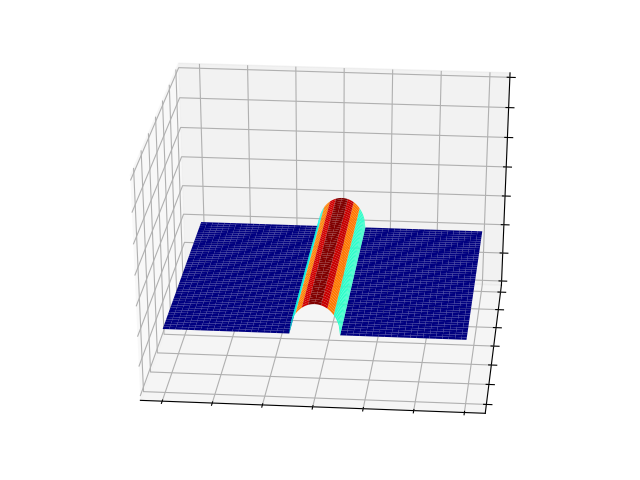
\includegraphics[width=\linewidth]{circular_trough}
      \caption{The graph of a cylindrical ridge of radius $r$,
			      	as given by $f(x,y)$ as given above.}
      \end{figure}
      
      
      We calculate the necessary partial derivatives of $f$ as follows:
      
      \begin{gather}
      \frac{\partial f}{\partial x} = \left(1, 0, \frac{-x}{\sqrt{r^2 - x^2}}\right)
      \quad , \quad
      \frac{\partial^2 f}{\partial x^2} = \left(0, 0, \frac{-r^2}{\left(\sqrt{r^2 - x^2}\right)^3}\right) \\
      \frac{\partial f}{\partial y} = \left(0, 1, 0\right)
      \quad , \quad
      \frac{\partial^2 f}{\partial y^2} = \frac{\partial^2 f}{\partial x \partial y} = 0
      \end{gather}
      The gauss map is given by
      \begin{gather}
      \nu(x,y) = \frac{\frac{\partial f}{\partial x} \times \frac{\partial f}{\partial y}}
      {\vnorm{\frac{\partial f}{\partial x} \times \frac{\partial f}{\partial y}}}
      = \left( \frac{x}{r} ,\; 0 ,\; \frac{\sqrt{r^2 - x^2}}{r} \right) \\
	  \implies
	  \frac{\partial \nu}{\partial x}
		  = \left(\frac{1}{r} \;,\; 0\;,\; \frac{-x}{r\sqrt{r^2-x^2}}\right)
		  \quad , \quad \frac{\partial \nu}{\partial y} = \left(0,0,0\right).
      \end{gather}
      
      We then calculate matrix elements of the Weingarten map's construction as given in
      \cref{hij_exactgraph} and \cref{gij_exactgraph} :
      \begin{align}
      [h_{ij}] = \frac{1}{\sqrt{1+h_x^2 + h_y^2}} \,  \Hess (h)
		       &= \frac{1}{\sqrt{1+\left(\frac{x^2}{r^2-x^2}\right)}}
		       \begin{bmatrix}
		       \frac{-r^2}{\sqrt{r^2 - x^2}^3} & 0 \\
			     0 & 0
		       \end{bmatrix} 
		       &= \begin{bmatrix}
		       \frac{-r}{r^2 - x^2} & 0 \\
		       0 & 0
		       \end{bmatrix} \\
		       [g_{ij}]^{-1} &= \begin{bmatrix} \frac{r^2 - x^2}{r^2} & 0 \\ 0 & 1 \end{bmatrix} \\
		       \implies \weinmat = [h_{ij}]	[g_{ij}]^{-1} &=
		       \begin{bmatrix}
		       \frac{-r}{r^2 - x^2} & 0 \\
		       0 & 0
		       \end{bmatrix} \begin{bmatrix} \frac{r^2 - x^2}{r^2} & 0 \\ 0 & 1 \end{bmatrix} \\
		       &= \begin{bmatrix} - \frac{1}{r} & 0 \\ 0 & 0 	\end{bmatrix}	       	
      \end{align}
      
      We see that $u_2 = (0,1)$ and $u_1 = (1,0)$ are eigenvectors for $\weinmat$ with respective eigenvalues
      $\kappa_2 = -\frac{1}{r} , \kappa_1 = 0$. Given the theorem of Olinde Rodriguez suggests that $u_2$ points in the direction of maximum curvature of the surface, $-\frac{1}{r}$, which is predictably in the direction directly perpendicular to the trough, whereas the direction of least curvature is along the trough and is $0$. The theorem of Meusnier suggests that the normal curvature $\kappa_2 = -\frac{1}{r}$ is reasonable-- any curve on the trough perpendicular to the ridge should have the curvature of a circle (the negative simply indicates that we are on the ``outside'' of the surface). Finally, we note that at the ridge of the trough is exactly where $\nabla f = 0$, and the Weingarten map is exactly the Hessian matrix there.
      
      \vcleanup{this was dropped in here. fix the transition}
      Viewing the surface in $\R^3$, we define the Hessian \vcomment{notation here, does it need to be an operator?} $\Hess$ of the surface $L$
      at a point $(x,y)$ on the surface as the matrix of its second partial derivatives:
      \begin{equation}
      \Hess(x,y) = \begin{bmatrix}
      L_{xx}(x,y) & L_{xy}(x,y) \\
      L_{yx}(x,y) & L_{yy}(x,y)
      \end{bmatrix}
      \end{equation}
      
      At any point $(x,y)$ we denote the two eigenpairs of $\Hess(x,y)$ as
      \begin{equation}
      \Hess u_i = \kappa_i u_i \; , \quad i = 1,2
      \end{equation}
      
	  \vcleanup{the eigenvectors of the Weingarten map are orthonormal. the eigenvectors of the hessian are also orthonormalizable. make the distinction!}
      where $\kappa_i$ and $u_i$ are known as the
      \textit{principal curvatures} and \textit{principal directions} \vcomment{fixthis} of $L(x,y)$, respectively, and we label such that $|\kappa_2| \ge |\kappa_1|$. Notably, $\Hess(x,y)$ is a real, symmetric matrix (since  $L_{xy} = L_{yx}$ and $L$ is a real function)and thus its eigenvalues are real and its eigenvectors are orthonormal to each other, as given by following lemma:
      
      % from burden and faires corollary 9.17
      \begin{lemma}[Principal Axis Theorem?]
      	Let $A$ be a real, symmetric matrix. The eigenvalues of $A$ are real and its eigenvectors are orthonormal to each other.
      \end{lemma}
      
      \begin{proof}
      	Let $x\ne 0$ so that $Ax = \lambda x$. Then 
      	\begin{align*}
      	\vnorm{Ax}_2^2 = \inner{Ax}{Ax}  &= (Ax)^{*} Ax \\
      	&= x^{*}A^{*}Ax = x^{*}A^T A x = x*A A x \\
      	&= x^{*} A \lambda x = \lambda x^{*} A x \\
      	&= \lambda x^{*} \lambda x = \lambda^2 x^{*} x = \lambda ^2 \vnorm{x}_2^2
      	\end{align*}
      	Upon rearrangement, we have
      	$\lambda^2 = \frac{\vnorm{Ax}_2^2}{\vnorm{x}_2^2} \ge 0 \implies \lambda $ is real.
      	
      	To prove that a set of orthonormalizable eigenvectors exists,
      	let $A$ be real, symmetric as above and consider the eigenpairs
      	$Av_1 = \lambda_1 v_1$, $Av_2 = \lambda_2 v_2$ with $v_1, v_2 \ne 0$.
      	\footnote{To simplify notation, we simplify our argument to consider two explicit eigenvectors only, since we're only concerned with the $2\times 2$ matrix $\Hess$
      		anyway.}
      	
      	In the case that $\lambda_1 \ne \lambda_2$, we have
      	\begin{align*}
      	(\lambda_1 - \lambda_2)v_1^T v_2 &= \lambda_1 v_1^T v_2 - \lambda_2 v_1^T v_2 \\
      	&= (\lambda_1 v_1)^T v_2 - v_1^T (\lambda_2 v_2) \\
      	&= (Av_1)^T v_2 - v_1^T (Av_2) \\
      	&= v_1^T A^T v_2 - v_1^T A v_2 \\
      	&= v_1^T A v_2 - v_1^T A v_2 = 0
      	\end{align*}
      	Since $\lambda_1 \ne \lambda_2$, we conclude that $v_1^T v_2 = 0$.
      	
      	In the case that $\lambda_1 = \lambda_2 =: \lambda$, we can define
      	(as in Gram-Schmidt orthogonalization) $u = v_2 - \frac{v_1^Tv_2}{v_1^Tv_1}v_1$.
      	This is an eigenvector for $\lambda=\lambda_2$, as
      	\begin{align*}
      	Au &= A\left(v_2 - \frac{v_1^Tv_2}{v_1^Tv_1} v_1\right) \\
      	&= A v_2 - \frac{v_1^Tv_2}{v_1^Tv_1} A v_1 \\
      	&= \lambda v_2- \frac{v_1^Tv_2}{v_1^Tv_1} \lambda v_1 \\
      	&= \lambda \left( v_2 - \frac{v_1^Tv_2}{v_1^Tv_1} v_1 \right) = \lambda u
      	\end{align*}
      	and is perpendicular to $v_1$, since
      	\begin{align*}
      	v_1^T u &= v_1^T\left(v_2 - \frac{v_1^Tv_2}{v_1^Tv_1}v_1\right) \\
      	&= v_1^T v_2 - \left(\frac{v_1^Tv_2}{v_1^Tv_1}\right) v_1^T v_1 \\
      	&= v_1^T v_2 - v_1^Tv_2 (1) = 0.
      	\end{align*}
      \end{proof}
      
      Thus we see that the two principal directions form an orthonormal frame at each point (x,y) within the continuous image $L(x,y)$.
      
      \vcomment{The following unverified (but intuitive) theorem is currently unnecessary but could be useful if I still want to implement the idea of tracking direction of eigenvectors along potential ridges, useful for filling in the ridge network. Like approximating the surface using derivatives.}
      The following is an \textbf{unverified claim} (which might be useful for later):
      The frame varies continuously along paths in $\R^2$
      except at points where $\Hess(x,y)$ is singular.
      To make this explicit:
      
      \begin{theorem}[Continuity of the leading principal direction]
      	Let $\theta: I:= [0,1] \to \R^2$ be a parametrized regular curve in $\R^2$ and
      	$H_\theta := \Hess_f  \circ \theta(t)$ be the matrix-valued function
      	% use the same notation as the Hessian before and cite the eqn. number from earlier
      	(where $\Hess_f$ is the $2\times 2$ Hessian of the smooth surface $f$)
      	Let $U:I \to \R^2$ be the implicitly-defined vector valued function s.t.
      	$U(t)$ is the leading eigenvector of $H_\theta$
      	(and therefore the leading principal direction of $f$). That is,
      	\begin{equation}
      	H_\theta \; U(t) = \lambda U(t) \quad \textrm{with}\quad \lambda = \rho(H_\theta)
      	\end{equation}
      	In other words, $\abs{\lambda} \ge \abs{\tilde{\lambda}}$ for any
      	$\tilde{\lambda} : H_\theta \; u = \tilde{\lambda} u$ for some $u \ne 0$.
      	
      	Then, $U(t)$ is continuous in $t$ whenever $H_f(t)$ is non-singular.
      	\vcomment{Maybe fix this so that the path avoids any nonsingular points?
      		$U(t)$ isn't even well-defined at such points anyway.}
      \end{theorem}
      \begin{proof}
      	First, we show that $U(t)$ is a well-defined function at all points $t$ where
      	$H_f(t)$ is non-singular.
      	\vtodo{FIX PROOF OR REMOVE}
      \end{proof}
      
      \vcomment{Need a transition} To we are interested in the differentiation of 2D images, we need a way
      to calculate the quantities of the previous section \vcleanup{tag}. We can simply extend these ideas of differentiation to the discrete domain.
    
\section{Calculating Derivatives of Discrete Images} 

	
	\begin{itemize}
		\item \vtodo{Describe taking gradient with divided difference.}
		\item \vtodo{Describe the situation: derivatives should be taken on Gaussian blur (equivalent to scale space development) [Lindeberg]. That is, you can take the derivative of either the convolved image, or you can take derivatives of the Gaussian itself, \textit{then} convolve.}
		\item \vtodo{Mention that derivatives can be taken in frequency space?}

%		Pseudocode for \texttt{np.gradient} which is used in calculating Hessian (code below)
%					\begin{verbatim}
%					gaussian_filtered = fftgauss(image, sigma=sigma)
%					Lx, Ly = np.gradient(gaussian_filtered)
%					Lxx, Lxy = np.gradient(Lx)
%					Lxy, Lyy = np.gradient(Ly)
%					\end{verbatim}	
		\end{itemize}
\vcomment{describe this no matter what. if you want to calculate the derivatives in frequency space,
	still describe this so you can compare the results.}
\vcleanup{Move scale space theory section before this.}


\section{The Frangi Filter} \label{sec:frangi}


    \subsection{Intro to Hessian-based filters}
	%Basic properties and observations. Why these filters make sense. Basic strengths and weaknesses.

        Hessian-based filters are a family of curvilinear filters that employ the Hessian and its eigenspaces
        to determine regions of significant curvature within an image.
        % as mentioned by Frangi, see Sato [13] and Lorenz [10] in their paper
        Several such filters exist --see Sato [13] and Lorenz[10]. These filters use information about the principal curvatures (eigenvalues of the Hessian) at each point to 
        
        
	\subsection{Implementation Details: Convolution Speedup via FFT}
	\vcomment{FIRST DESCRIBE HOW YOU NEED DERIVATIVES}
	
	As described above, the actual computation of derivatives is achieved via convolution with a gaussian. In practice, this is very slow for large scales. We instead, we perform a fast Fourier transform, which offers a speedup of $N^2$ operations vs $\mathscr{O}\left(n\cdot \log_2n\right)$ operations \vcomment{extend to 2D}

\vcleanup{Fix this part of the outline}
\section{Fourier Transforms}
	\subsubsection{Fourier Transform of a continuous 1D signal}
	
	\vcomment{start with 1D but then extend/rewrite}
	
	A periodic signal (real valued function) $f(t)$ of period $T$ can \vcomment{justify?} be expanded in an infinite basis as follows:
	
	\begin{equation}
		f(t) = \sum_{-\infty}^{\infty} c_n e^{i\frac{2\pi n}{T}t} \;,\quad
			c_n = \frac{1}{T}\int_{-T/2}^{T/2} f(t) e^{-i\frac{2\pi n}{T}t} dt
			\end{equation}
	
	The Fourier transform of a 1D continuous function is defined by
	\begin{equation} \label{1D-CFT}
		F(\mu) := \FT\{f(t)\} \;=\; \int_{-\infty}^{\infty} f(t) e^{i2\pi \mu } dt
	\end{equation}
	
	It can be shown \vcomment{justify?} that an inverse transform will then recover our original signal:
	\begin{equation} \label{1D-ICFT}
		f(t) = \FT^{-1}\left\{F(\mu)\right\} = \int_{-\infty}^{\infty} F(\mu) e^{i2\pi \mu t} dt
	\end{equation}
	
	Together, \cref{1D-CFT} and \cref{1D-ICFT} are referred to as the \textit{Fourier transform pair} of the signal $f(t)$. 
	
	\subsubsection{Fourier Transform of a Discrete 1D signal}
	
	We wish to develop the Fourier transform pair for a discrete signal. We frame the situation
	as follows: A continuous function $f(t)$ \vcomment{right now, with domain $\R$} is represented as the sampled function $\tilde{f}(t)$ by multiplying it by a sampling function (also referred to
	in DIP-GW as an impulse function), an infinite series of discrete impulses with equal spacing $\Delta T$:
	
	\begin{equation} \label{1D-sampling-function}
	s_{\Delta T}(t) = \sum_{n=-\infty}^{\infty} \delta[t - n\Delta T] \;,\quad
	\delta[t] = \begin{cases} 1 \;,\; & t=0 \\ 0 \;,\;& t \ne 0 \end{cases}
	\end{equation}
	
	where $\delta[t]$ is the discrete unit impulse.
	
	The discrete sample $f(t)$ is then constructed from $f(t)$ by
	\begin{equation} \label{1D-discrete-sample}
	\tilde{f}(t) = f(t) s_{\Delta T}(t)
	\end{equation}
	
	From this (and actually the convolution theorem) we can calculate $\tilde{F}(t)$. \vtodo{Derive this. There's some groundwork here to copy between 213-220. We don't need the sampling theorem, since our signal is given as-is... i think}.
	
	\subsubsection{1D Discrete Fourier Transform (DFT)}
	
	Given the discrete signal $\tilde{f}$, we construct the transform
	$\tilde{F}(\mu) = \FT\{\tilde{f}(t)\}$. by simply transforming the definition \cref{1D-discrete-sample}.
	
	\vcomment{supress derivation but do explain $f_n$ notation / cleanup}
	
	\begin{equation} \label{1D-DFT-transform}
	\tilde{F}(\mu) = \sum_{n=-\infty}^{\infty} f_n e^{-i 2\pi \mu n \Delta T} \;,\quad
		f_n = \tilde{f}(n) = f(n\Delta T)
	\end{equation}
	
	The transform is a continuous function with period $1 / \Delta T$. 
	
		\begin{itemize}
			\item \vtodo{find image processing papers that find hessian from FFT / who uses this?}
			\item \vtodo{with above: downsides?}
			\item \vtodo{side by side comparison in a toy example and/or a real problem?}
		\end{itemize}
		
		\subsubsection{2D Discrete Fourier Transform Convolution Theorem}\vcomment{the following was adapted in a large part from DFT: an owner's manual. cite? DIP-DW just proves the continous version (in 1D) and then asserts that it works for discrete variables too.}
		
		\vcleanup{get consistent notation--either have the discrete signals be notated as  $\tilde{f}(x,y)$ or $f[x,y]$ or instead comment that it's understood}
		\begin{theorem}[2D DFT Convolution Theorem] 
			\vcomment{develop the 2-D DFT from Sec. 4.3 4.4 from DIP-GW (see p235).}
		Given two discrete functions are sequences with the same length \vtodo{don't gloss over this} \vcomment{If they're not actually the same length, DIP-GW suggests to make the final length at least $P = A+C-1$ and $Q = B+D-1$ in the case that the sizes are $A\times B$ and $C\times D$ for $f(x,y)$ and  $h(x,y)$ respectively. Not sure if that matters.}, that is:
		$f(x,y)$ and $h(x,y)$ for integers $0 < x < M$ and $0 < y < N$, we can take the discrete fourier transform (DFT) of each:
		\begin{align}
		F(u,v) := \mathcal{D}\{f(x,y)\} &=
						\sum_{x=0}^{M-1} \sum_{y=0}^{N-1} f(x,y)
						e^{-2\pi i \left(\frac{ux}{M} + \frac{vy}{N}\right)} \\	
		   H(u,v) := \mathcal{D}\{h(x,y)\} &=
						\sum_{x=0}^{M-1} \sum_{y=0}^{N-1} h(x,y)
						e^{-2\pi i \left(\frac{ux}{M} + \frac{vy}{N}\right)}
		\end{align}
		
		and given the convolution of the two functions
		\begin{equation}
		\left(f \star h\right)(x,y) = \sum_{m=0}^{M-1} \sum_{n=0}^{N-1} f(m,n)h(x-m,y-n)
		\end{equation}
		
		then $\left(f \star h\right)(x,y)$ and $MN\cdot F(u,v)H(u,v)$ are transform pairs, i.e.
		\begin{equation}
		\left(f \star h\right)(x,y) = \mathcal{D}^{-1}\left\{MN\cdot F(u,v)H(u,v)\right\}
		\end{equation}
		\end{theorem}
		
		
		The proof follows from the definition of convolution, substituting in the inverse-DFT of $f$ and $h$, and then rearrangement of finite sums.
		\begin{proof}
		\begin{align}
		\left(f \star h\right)(x,y) &= \sum_{m=0}^{M-1} \sum_{n=0}^{N-1} f(m,n)h(x-m,y-n) \\
		&= \sum_{m=0}^{M-1} \sum_{n=0}^{N-1}
		\left(\sum_{p=0}^{M-1} \sum_{q=0}^{N-1} F(p,q)
			e^{2\pi i \left(\frac{mp}{M} + \frac{nq}{N}\right)}\right)
			\left(\sum_{u=0}^{M-1} \sum_{v=0}^{N-1} H(u,v)
			e^{2\pi i \left(\frac{u(x-m)}{M} + \frac{v(y-n)}{N}\right)} \right) \\
		&= \left(\sum_{u=0}^{M-1} \sum_{v=0}^{N-1} H(u,v)
			e^{2\pi i \left(\frac{ux}{M} + \frac{vy}{N}\right)}\right)
			\left(\sum_{p=0}^{M-1} \sum_{q=0}^{N-1} F(p,q)
			\left(\sum_{m=0}^{M-1} e^{2\pi i \left(\frac{m(p-u)}{M}\right)}\right)
			\left(\sum_{n=0}^{N-1} e^{2\pi i \left(\frac{n(q-v)}{N}\right)}\right)\right) \\
			&= \left(\sum_{u=0}^{M-1} \sum_{v=0}^{N-1} H(u,v)
			e^{2\pi i \left(\frac{ux}{M} + \frac{vy}{N}\right)}\right)
			\left(\sum_{p=0}^{M-1} \sum_{q=0}^{N-1} F(p,q)
			\left( M \cdot \hat{\delta}_M(p-u) \right)
			\left( N \cdot \hat{\delta}_M(q-v)\right)\right) \\
			&= \left(\sum_{u=0}^{M-1} \sum_{v=0}^{N-1} H(u,v)
			e^{2\pi i \left(\frac{ux}{M} + \frac{vy}{N}\right)}\right)
			\cdot M N F(u,v) \\
			&=MN \cdot \sum_{u=0}^{M-1} \sum_{v=0}^{N-1} F(u,v) H(u,v)
			e^{2\pi i \left(\frac{ux}{M} + \frac{vy}{N}\right)} \\
			&= MN \cdot \mathcal{D}^{-1}\left\{ FH\right\}
		\end{align}
		
		where
		\begin{equation} \label{delta_multiple}
			\hat{\delta}_N (k) = \begin{cases}
				1 & \text{when } k = 0 \mod N \\
				0 & \text{else}
				\end{cases}
		\end{equation}
	\end{proof}
	Above, we make use of the following lemma \vcomment{add this before DFT convolution theorem and embed the definition of $\hat{\delta}_N$ inside}
	\begin{lemma}
	Let $j$ and $k$ be integers and let $N$ be a positive integer. Then
	\begin{equation} \label{dft_conv_lemma}
		\sum_{n=0}^{N-1} e^{2\pi i\left(\frac{n(j-k)}{N}\right)} =  N \cdot \hat{\delta}_N(j-k) 
		\end{equation}
		\end{lemma}
		\begin{proof}
		
		Consider the complex number $e^{2\pi i (j-k)/N}$. Note first that this is an $N$-th root of unity, since
		\[
		\left(e^{2\pi i (j-k)/N}\right)^N = e^{2\pi i (j-k)} = \left(e^{2\pi i}\right)^{(j-k)}
		= 1^{(j-k)} = 1
		\]
	
	In other words, $e^{2\pi i n(j-k)/N}$ is a root of $z^N -1 = 0$, which we can factor as
	\begin{equation}
	z^N -1 \;=\; (z-1)\left(z^{n-1} + \cdots + z + 1\right) \;=\; (z-1)\sum_{n=0}^{N-1} z^n .
	\end{equation}

thus giving us
\begin{equation} \label{dft_conv_lemma_factors}
	0 = \left(e^{2\pi i(j-k)/N} - 1\right) \sum_{n=0}^{N-1} e^{2\pi i n(j-k)/N}
	\end{equation}
	
To prove the claim in \cref{dft_conv_lemma}, we consider two cases: First, if $j-k$ is a multiple of $N$, we of course have $e^{2\pi i n(j-k)/N} = \left(e^{2\pi i}\right)^{n(j-k)/N} = 1$  and thus the left side of \cref{dft_conv_lemma} reduces to 
\[
\sum_{n=0}^{N-1} \left(e^{2\pi i}\right)^{n(j-k)/N} = \sum_{n=0}^{N-1} \left(1\right) = N
\].

In the case that $j-k$ is \textit{not} a multiple of $N$, we refer to \cref{dft_conv_lemma_factors}.
The first factor is not zero since, $\left(e^{2\pi i (j-k)/N}\right) \ne 1$ (simply since $(j-k)/N$ is not an integer), and thus it must be that the second factor is 0:
\[
\sum_{n=0}^{N-1} \left(e^{2\pi i (j-k)/N}\right)^n = 0\]
	
	We can combine these two cases by invoking the definition of \cref{delta_multiple}, giving us the result.
		\end{proof}
				
		\subsubsection{FFT}
		 \vcomment{use DIP-GW p298}
		As noted, the above result applies to the Discrete Fourier Transform. As noted, we actually achieve a convolution speedup using a Fast Fourier Transform (FFT) instead. We follow the developments of DIP-GW \vcomment{should I? or just link? or fix notation? or do for 2D at the same time}. For clarity, we present the following theorems which allow a framework to calculate a 2D Fourier transforms quickly.
		
		
		First, a 2D DFT may actually be calculated via two successive 1D DFTs, which can be
		seen through a basic rearrangement, as follows:
		
		\begin{align}
		F(\mu,\nu) &= \sum_{x=0}^{M-1} \sum_{y=0}^{N-1} f(x,y) e^{-i2\pi \left(\mu x/M + \nu y/N\right)} \\
			   &= \sum_{x=0}^{M-1} e^{-i2\pi \mu x/M} \left[ \sum_{y=0}^{N-1} f(x,y)e^{-i2\pi \nu y/N} \right] \\
			   &= \sum_{x=0}^{M-1} e^{-i2\pi \mu x/M} \FT_x\{ f(x,y)\} \\
			   &= \FT_y\{\FT_x \{f(x,y)\} \}
		\end{align}
		
		where $\FT_{x'}$ refers to the 1D discrete Fourier transform of the function with respect to
		the variable $x'$ only.
		
		Thus, to calculate the fourier transform $F(u,v)$ at the point $u,v$
		requires the computation of the transform of length $N$ for each iterated point $x \in 0..M-1$. Thus there are $MN$ complex multiplications and $(M-1)(N-1)$ complex additions in this sequence required for each point $u,v$ that needs to be calculated. Overall, for all points that need to be calculated, the total order of calculations is on the order of $(MN)^2$ \vcomment{rectify this, is it really caused by the number of $u,v$ points that need calculating?}. (Note: the values of $e^{-i2\pi m/n}$ can be provided by a lookup table rather than ad-hoc calculation \vcomment{source?}.
		
		We now show that a considerable speedup can be achieved through elimination of redundant calculations. In particular, we wish to show that the calculation of a 1D DFT of signal length $M=2^n, n \in \Zpos$ can be reduced to calculating two half-length transforms and an additional $M/2 = 2^{n-1}$ calculations.
		
		\vcomment{we follow DIP-GW variable conventions, which I think are dumb}
		
		To "simplify" our notation we will use a new notation for the Fourier kernels/basis functions.
		Let the 1D Fourier transform be given by
		
		\begin{equation} \label{FFT-defineW}
		F(u) = \sum_{x=0}^{M-1} f(x) W_M^{ux},\quad \textrm{where} \quad W_m := e^{-i2\pi/m}
		\end{equation} 
		
		We'll define $K \in \Zpos : 2K = M = 2^n$ (i.e. $K = 2^{n-1})$.
		
		We use this to rewrite the series in \cref{FFT-defineW} and split it into odd and even entries in the summation
		
		\begin{align}
		F(u) &= \sum_{x=0}^{2K-1} f(x) W_{2K}^{ux} \\
			 &= \sum_{x=0}^{K-1} f(2x) W_{2K}^{u(2x)}
				 + \sum_{x=0}^{K-1} f(2x+1) W_{2K}^{u(2x+1)} \label{FFT-oddevensplit}
		\end{align}
		
		We'll get a few identities out of the way (where $m, n, x \in \Zpos$ arbitrary).
		
		\vcomment{this fixes an issue in DIP-GW where the identities were provided in terms of $M$ instead of arbitrary $m$, where the proof uses the results for some value other than $M$ anyway}
		\begin{gather} \label{fft-kernelidentities}
		W_{(2m)}^{(2n)} = e^{\frac{-i2\pi(2m)}{2m}} = e^{\frac{-i2\pi m}{n}} = W_{m}^{n} \\
		W_{m}^{(u+m)x} = e^{\frac{-i2\pi(u+m)x}{m} } = e^{\frac{-i2\pi unx}{m}} e^{\frac{-i2\pi mx}{m}}
					= e^{\frac{-i2\pi ux }{m}} (1) = W_m^{ux} \\
		W_{2m}^{(u+m)} = e^{\frac{-i2\pi(u+m)}{2m}} = e^{\frac{-i2\pi ux}{2m}} e^{-i\pi}
					 = W_{2m}^{u} e^{-i\pi} = - W_{2m}^{u}
		\end{gather}

Thus we can rewrite \cref{FFT-oddevensplit} as
\begin{align}
F(u)  &= \sum_{x=0}^{K-1} f(2x) W_{2K}^{2ux} + \sum_{x=0}^{K-1} f(2x+1) W_{2K}^{2ux} W_{2K}^{u} \\
\Longrightarrow \quad F(u) &= \left(\sum_{x=0}^{K-1} f(2x) W_{K}^{ux}\right)
	 + \left(\sum_{x=0}^{K-1} f(2x+1) W_{K}^{ux}\right) W_{2K}^{u}
		 \label{fft-oddeven-parens}
\end{align} 

The major advance comes via using the identities \cref{fft-kernelidentities} \vcleanup{fix multitag} to consider the Fourier transform $K$ 
frequencies later \vcomment{wording?}:
\begin{align}
F(u+K) &= \left(\sum_{x=0}^{K-1} f(2x) W_{K}^{(u+K)x}\right)
+ \left(\sum_{x=0}^{K-1} f(2x+1) W_{K}^{(u+K)x}\right) W_{2K}^{(u+K)}\\
\Longrightarrow F(u+K) &= \left(\sum_{x=0}^{K-1} f(2x) W_{K}^{ux}\right)-\left(\sum_{x=0}^{K-1} f(2x+1)W_K^{ux}\right) W_K^{u}
\label{fft-oddeven-parens-plusK}
\end{align}


Comparing \cref{fft-oddeven-parens} and \cref{fft-oddeven-parens-plusK}, we see that the expressions within parentheses are identical.
	What's more, these parentetical expressions are functionally identical to discrete fourier transforms themselves! Let's notate them as follows:
	\begin{align} \label{fft-oddeven-subdfts}
	\DFT_u\{f_{\mathrm{even}}(t)\} &:= \sum_{x=0}^{K-1} f(2x)W_K^{ux} \\
	\DFT_u\{f_{\mathrm{odd}}(t)\} &:= \sum_{x=0}^{K-1} f(2x+1)W_K^{ux}
	\end{align}
	
	If we're calculating an $M$ point transform \vtodo{vocabulary also how many frequencies do we calculate? same as \# samples? what do we need?} (i.e. we're wishing to
	calculate $F(1), ... , F(M))$, once we've calculated the first $K$ discrete frequencies (i.e. $F(1), .. , F(K))$ we may simply reuse the two values we've calculated in \cref{fft-oddeven-subdfts} to calculate the next $F(K+1),..,F(K+K) = F(M)$. Since each expression in parentheses involves $K$ complex multiplications and $K-1$ complex additions, we are effectively saving $K(2K-1)$ calculations in computing the entire spectrum  $F(1), ..,  F(M)$. When $M$ is large, the payoff is undeniable.

In fact, through counting calculations and then doing a proof by induction, we can show that the effective number of calculations is given by $M\log_2{M}$. \vtodo{finish this}.

Of course, since \cref{fft-oddeven-subdfts} are DFTs themselves, there's nothing stopping us from reiterating this procedure; if $M$ is substantially large, we can just as easily repeat this process a few times.

Of course, our development was for $1D$.  We can extend this to $2D$ by taking note of \vcleanup{cite previous section or move section here.}
	
The one caveat is that the above development was for transforming sequences whose lengths are perfect powers of $2$. Since our inputs have no reason to be this, we need to adjust for this. The explanation is \vtodo{probably} that you just do the part that's a power of 2 and  then do the rest manually or pick a different power. See \vtodo{find out how fft-pack does this}


The inverse DFT is actually a DFT of a modified function, see \vtodo{cite DIP-GW here or show that}. \vtodo{check how fftpack does this}

\hrulefill
\section{Linear Scale Space Theory}
	\vcomment{this is all as cited in GSST book (see starting in sec 6.3.1).
		as mentioned there, this is analogous to a discrete development
		(lindeberg 1990 lindeberg 1991 lindeberg 1994c lindeberg 1994e)}
	
	Koenderink showed/asserted that "any image can be embedded in a one-parameter family of derived images (with resolution as the parameter) in essentially only one unique way" given a few of the so-called \textit{scale space axioms}. They showed in particular that any such family must satisfy the heat equation
	\begin{equation}
		\Delta K(x,y,\sigma) = K_\sigma (x,y,\sigma) 
		\;\text{for}\; \sigma \ge 0
		\;\text{such that}\; K(x,y, 0) = u_0(x,y).
		\end{equation}
		
		where $K: \R^3 \to \R $ and  $u_0: \R^2 \to \R: $ is the original image (viewed as a continuous surface) and $\sigma$ is a resolution parameter.
	Much work has been done to formalize this approach. There is a long list of desired properties
	quoted from gsst. goal is to try to find a minimal subset of axioms and show that other desired properties follow.
	
	
\subsection{Axioms}
	To make matters manageable, [PEOPLE] have taken the approach of requiring the one-parameter family of scaled images to be generated by an operation.
	
	\subsection{Linear-shift invariance}
		This requires that the generator is convolution by some kernel. Show or proclaim.
		Shift-invariant means that no position in the original signal is favored (makes sense, this should apply to any image.)
	
	\subsubsection{Rotational invariance}
		Similar to above, no favoritism to directionality.
	
	\subsubsection{Semigroup property}
		They stack (no preferred scale)
	
	\subsubsection{Causality condition}
		No ``spurious resolution'' can be generated as parameter increases. \vcomment{FIX NOTATION}
		If $K(x_0,y_0;z_0)$ is a local maximum (in space)
			(i.e. $\nabla_{x,y}K(x_0,y_0; z_0) = 0 \;,\; \Delta_{x,y} K(x_0,y_0;z_0) < 0$ ),
			then an increase in scale can only weaken this peak, i.e.
			\begin{equation}
			z_0 > z_1 \implies K(x_0,y_0;z_0) \ge K(x_0,y_0;z_1)
			\end{equation}
		Similarly, if $K(x_0,y_0;z_0)$ is a local minimum (in space), (i.e. $\nabla_{x,y}K(x_0,y_0; z_0) = 0 \;,\; \Delta_{x,y} K(x_0,y_0;z_0) > 0$ ),
		then an increase in scale cannot make such a valley more profound, i.e.
		\begin{equation}
		z_0 > z_1 \implies K(x_0,y_0;z_0) \le K(x_0,y_0;z_1)
		\end{equation}
	
	This implies that no image feature is sharpened by an decrease and resolution--the only result is a flattening out of the image as scale parameter $z$ tends to infinity.s
	
	
	\subsubsection{Linearity of generator}
	``Linearity implies that all-scale space properties valid for the original signal will transfer to its derivatives. Hence, there is no commitment to certain aspects of image structure, such as the zero-order representation, or its first- or second-order derivatives.''
	\vcomment{this is dubious, as mentioned by JvB}


\subsection{Necessity of convolution}
	Where is this.
\subsection{Uniqueness of the Gaussian Kernel}
	Proved \vcomment{however artificially} by Koenderink [1984] and Babaud [1986] that such an axiomatic foundation requires that the family is generated by convolution with a kernel. The remainder of the development is to the determine that the kernel is exactly the Gaussian.
	 
	 \vtodo{TODO:
		JUST EVEN OUT THE ABOVE.
		FIND SOMETHING TO JUSTIFY CONVOLUTION.
		CITATIONS FOR LATER FORMULATIONS.
		BUILD UP HEAT EQUATION (HOWEVER RIGOROUSLY YOU CAN).
		SHOW NECESSITY OF GAUSSIAN (OR DON'T).
	}
		

	 To this, show that:
		 \begin{itemize}
		 	\item a kernel satisfying the above axioms must satisfy the heat equation
		 	\item the gaussian kernel satisfies that.
		 	\item gaussian kernel is the only kernel that works (koenderink paper?)
		 \end{itemize}


\subsection{$G_\sigma \star u_0$ solves the heat equation}
	given $u_0$ as a continuous image (unscaled), we construct PDE with this as a boundary condition.
	
	\begin{equation}
		u: \R^2 \supset \Omega \to \R \; \textrm{with} \; u(\bm{x},t) : \;
			\begin{cases}
				\frac{\partial u}{\partial t} (\bm{x}, t) = \Delta u(\bm{x},t) & ,\; t \ge 0 \\
				u(\bm{x},0) = u_0(\bm{x}) 
			\end{cases}
		\end{equation}

	We show that
	\begin{equation}
		u(\bm{x},t) = \left(G_{\sqrt{2t}} \star u_0 \right)(\bm{x})
	\end{equation}
	solves (the above tagged equation), where
	\[
		G_\sigma := \frac{1}{2\pi \sigma^2} e^{\left(-\abs{x}^2 / (2\sigma^2)\right)}
	\]
	First, we need a quick lemma regarding differentiation a continuous convolution.
	\begin{lemma} \label{dconvolution}
		Derivative of a convolution is the way that it is (obviously rewrite this).
	\end{lemma}
	\begin{proof}
		For a single variable,
		\begin{align}
		\frac{\partial}{\partial \alpha} \left[ f(\alpha) \star g(\alpha) \right]
		&= \frac{\partial}{\partial \alpha} \left[ 
		\int f(t) g(\alpha - t) dt \right] \\
		&=  \int f(t) \frac{\partial}{\partial \alpha}\left[ g(\alpha - t)  \right] dt \\
		&=  \int f(t) \left(\frac{\partial g}{\partial \alpha}\right) g(\alpha - t) dt \\
		&=  f(\alpha) \star g'(\alpha)
		\end{align}
		By symmetry of convolution we can also conclude 
		\[\frac{\partial}{\partial \alpha} \left[ f(\alpha) \star g(\alpha) \right]
		= f'(\alpha) \star g(\alpha)
		\]
		
		If $f$ and $g$ are twice differentiable, we can compound this result to show a similar statement holds for second derivatives, and then, given the additivity of convolution,
		we may conclude
		\begin{equation}
		\Delta \left(f \star g \right) = \Delta(f) \star g = f \star \Delta(g) 
		\end{equation} 
	\end{proof}
	\begin{theorem}
		$u(\bm{x},t) = \left(G_{\sqrt{2t}} \star u_0 \right)(\bm{x})$ solves the heat equation.
	\end{theorem}
	\begin{proof}
		We focus on the particular kernel
		\[
			G_{\sqrt{2t}} = \frac{1}{4\pi t} e^{\left(-\abs{x}^2 / (4t)\right)}
			\]
	
	
	Then
	\begin{align}
	\frac{\partial u}{\partial t} (\bm{x}, t)
		&= \frac{\partial}{\partial t} \left(G_{\sqrt{2t}}(\bm{x},t) \star u_0(\bm{x})\right)  \\
		&= \frac{\partial}{\partial t} \left(G_{\sqrt{2t}}(\bm{x},t)\right) \star u_0(\bm{x})  \\
		&= \frac{\partial}{\partial t} \left(
			\frac{1}{4\pi t} e^{\left(-\abs{x}^2 / (4t)\right)} \right) \star u_0(\bm{x}) \\
		&= \left[
		-\frac{1}{4\pi t^2} e^{\left(-\abs{x}^2 / (4t)\right)}
			+ \frac{1}{4\pi t}\left(\frac{-\abs{x}^2}{4t^2}\right) e^{-\abs{x}^2 / (4t)}
			\right] \star u_0(\bm{x}) \\
			&= -\frac{1}{4t^2} \left( e^{\left(-\abs{x}^2 / (4t)\right)} 
					+ \abs{\bm{x}}^2 G_{\sqrt{2t}}(\bm{x},t)
						\right) \star u_0(\bm{x})
	\end{align}
	and from the previous lemma,
	\[
	\Delta u(\bm{x}, t) = \Delta\left( G_{\sqrt{2t}} \star u_0(\bm{x})\right)
						= \Delta\left( G_{\sqrt{2t}} \right)\star u_0(\bm{x})
	\]
	
	We explicitly calculate the Laplacian of $G_{\sigma}(x,y) = A \exp(-\frac{x^2 + y^2}{2\sigma^2})$ as follows:
	
	\begin{align*}
	\frac{\partial}{\partial x} G_{\sigma}(x,y)
		&= A \left( \frac{-2x}{2\sigma^2}\right) \exp\left(-\frac{x^2 + y^2}{2\sigma^2}\right) \\
		\implies \frac{\partial^2}{\partial^2 x} G_{\sigma}(x,y)
		&= A \cdot \frac{\partial}{\partial x}
		\left[ - \frac{x}{\sigma^2} \exp\left(-\frac{x^2 + y^2}{2\sigma^2}\right) \right] \\
		&= A \left[ - \frac{1}{\sigma^2} \exp\left(-\frac{x^2 + y^2}{2\sigma^2}\right) 
			+ \frac{x}{\sigma^2} \cdot \frac{2x}{2\sigma^2} \exp\left(-\frac{x^2 + y^2}{2\sigma^2}\right) \right] \\
			&= A \exp\left(-\frac{x^2 + y^2}{2\sigma^2}\right)
				\left[ - \frac{1}{\sigma^2} + \frac{x^2}{\sigma^4} \right] \\
				&= \frac{1}{\sigma^2} G_\sigma(x,y)  \left[ \frac{x^2}{\sigma^2} - 1\right]
	\end{align*}
	
	By symmetry of argument we also may conclude
	\[
	\frac{\partial^2}{\partial y^2} G_{\sigma}(x,y) = \frac{1}{\sigma^2} G_\sigma(x,y)  \left[ \frac{y^2}{\sigma^2} - 1\right]
	\]
	
	and so
	
	\begin{equation}
	\Delta G_\sigma(x,y) =
		\frac{\partial^2}{\partial x^2} \left(G_{\sigma}\right)
		+ \frac{\partial^2}{\partial y^2} \left(G_{\sigma}\right)
		= \frac{1}{\sigma^2} G_\sigma(x,y) \left[ \frac{x^2 + y^2}{\sigma^2} - 2\right] 
	\end{equation}
	Then, given \cref{dconvolution}, we conclude
	\begin{equation}
	\Delta \left[ G_\sigma(x,y) \star u_0(x,y) \right] 
	= \left(\frac{1}{\sigma^2} G_\sigma(x,y) \left[ \frac{x^2 + y^2}{\sigma^2} - 2\right]\right) \star u_0(x,y)
	\end{equation}
	
	For particular choices of $\sigma(t) = \sqrt{2t}$ and $A = \frac{1}{4\pi t}$,
	we see 
	\begin{align}
		\Delta \left[ G_{\sqrt{2t}}(x,y) \star u_0(x,y) \right] 
		&= \left(\frac{1}{2t} G_{\sqrt{2t}}(x,y) \left[ \frac{x^2 + y^2}{2t} - 2\right]\right) \star u_0(x,y) \\
		&= \left(G_{\sqrt{2t}}(x,y) \left[ \frac{x^2 + y^2}{4t^2} - \frac{1}{t}\right]\right) \star u_0(x,y)
	\end{align}
	We then calculate the time derivative,
	using our particular choice of $\sigma(t) = \sqrt{2t}$ and $A = \frac{1}{4\pi t}$ as:
	
	\begin{align}
	\frac{\partial}{\partial t} \left[ G_{\sigma(t)}(x,y) \star u_0(x,y) \right]
	&= \frac{\partial}{\partial t} \left[ G_{\sigma(t)}(x,y) \right] \star u_0(x,y) \\
	&= \frac{\partial}{\partial t} \left[ G_{\sqrt{2t}}(x,y)\right] \star u_0(x,y) \\
	&= \frac{\partial}{\partial t} \left[
	\frac{1}{4\pi t} \exp\left(-\frac{x^2 + y^2}{4t}\right) \right] \star u_0(x,y) \\
	&= \left[ -\frac{1}{4\pi t^2} \exp\left(-\frac{x^2 + y^2}{4t}\right) + 
	\frac{1}{4\pi t}\left( \frac{x^2 + y^2}{4t^2} \exp\left(-\frac{x^2 + y^2}{4t}\right)\right)
		\right] \star u_0(x,y) \\
		&= \left(G_{\sqrt{2t}}(x,y) \left[ \frac{x^2 + y^2}{4t^2} -\frac{1}{t}\right]\right) \star u_0(x,y)
	\end{align}

	Combining these results, we find that
	\begin{equation}
	\frac{\partial}{\partial t} \left[ G_{\sqrt{2t}} \star u_0 \right]
	= \Delta \left[ G_{\sqrt{2t}} \star u_0 \right] 
	\end{equation}
	
	as desired. \end{proof}
\hrulefill
\subsection{Alternative formulations of Scale Space Theory}
	Mention discrete treatments, mention relaxation of some of the dubious axioms.
\section{Morphology}
	Methods of merging multiscale methods.
	
	
\hrulefill

\section{Overview of Frangi vesselness measure}

\vcleanup{move to next session? or cover any necessary math here}

The Frangi filter \cite{frangi1998multiscale} is a widely used \vcomment{citation needed} Hessian-based filter used to detect curvilinear structures in images.  It was orignally developed for images such as MRIs and it excels in that context. It essentially relies on measuring eigenvalues of the Hessian $\Hess_\sigma(x,y)$ at some particular scale $\sigma$ at each point $(x,y)$ in the image.

The procedure for a single scale in a 2D image is as follows:

Let $\lambda_1, \lambda_2$ be the two eigenvalues of the Hessian, ordered such that $\abs{\lambda_1} \leq \abs{\lambda_2}$, where

\begin{equation} \label{frangivesselnessmeasure}
V_0(\sigma) = \begin{cases}
0 & \text{if} \quad \lambda_2 > 0 \\
\exp\left(-\frac{R^2}{2\beta^2}\right)
\left(1 - \exp(-\frac{S^2}{2c^2})\right) & \text{else}
\end{cases} \end{equation}
where
\begin{equation}
R := \lambda_1 / \lambda_2
\quad \textrm{and} \quad 
S := \sqrt{\lambda_1^2 + \lambda_2^2}
\end{equation}
and $\beta$ and $c$ are tuning parameters. Before we discuss appropriate values for $\beta$ and $c$, we first seek to highlight the significance of \cref{frangivesselnessmeasure}.



